\section{Starting expVIP web server}\label{starting-expvip-web-server}

Once the data is loaded, you can visualise the the expression in the
expVIP virtual machine.

\begin{enumerate}
\def\labelenumi{\arabic{enumi}.}
\itemsep1pt\parskip0pt\parsep0pt
\item
  Double click on \lstinline!start_expvip_server.sh!
  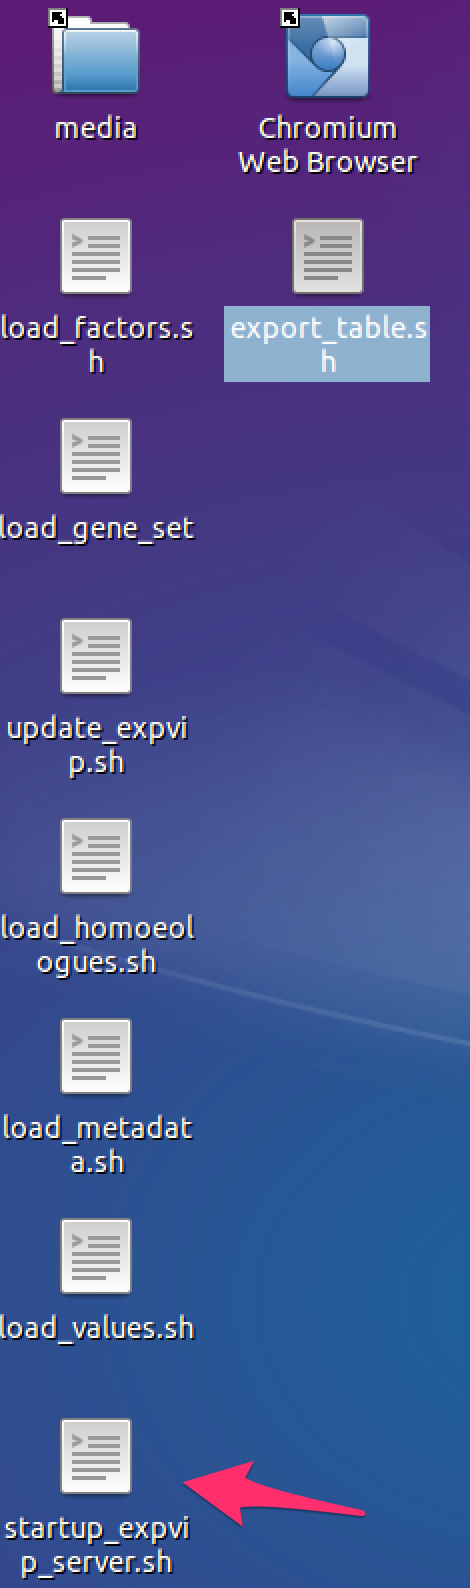
\includegraphics{images/StartupServer01.png}
\item
  Click on \lstinline!Execute on terminal!
  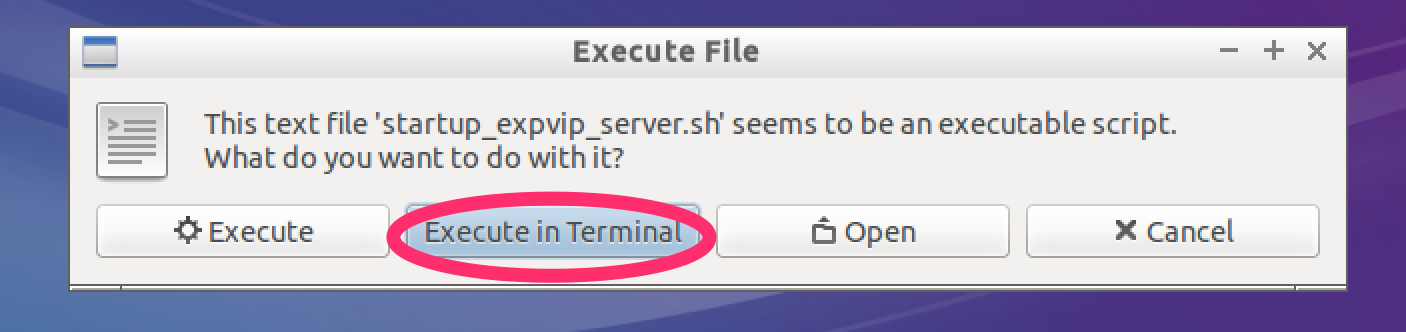
\includegraphics{images/StartupServer02.png}
\item
  Wait for the webserver to start. You know it is ready when the line
  \lstinline!WEBrickHTTPServer#start: pid=xxxx port=3000! appears in the
  console 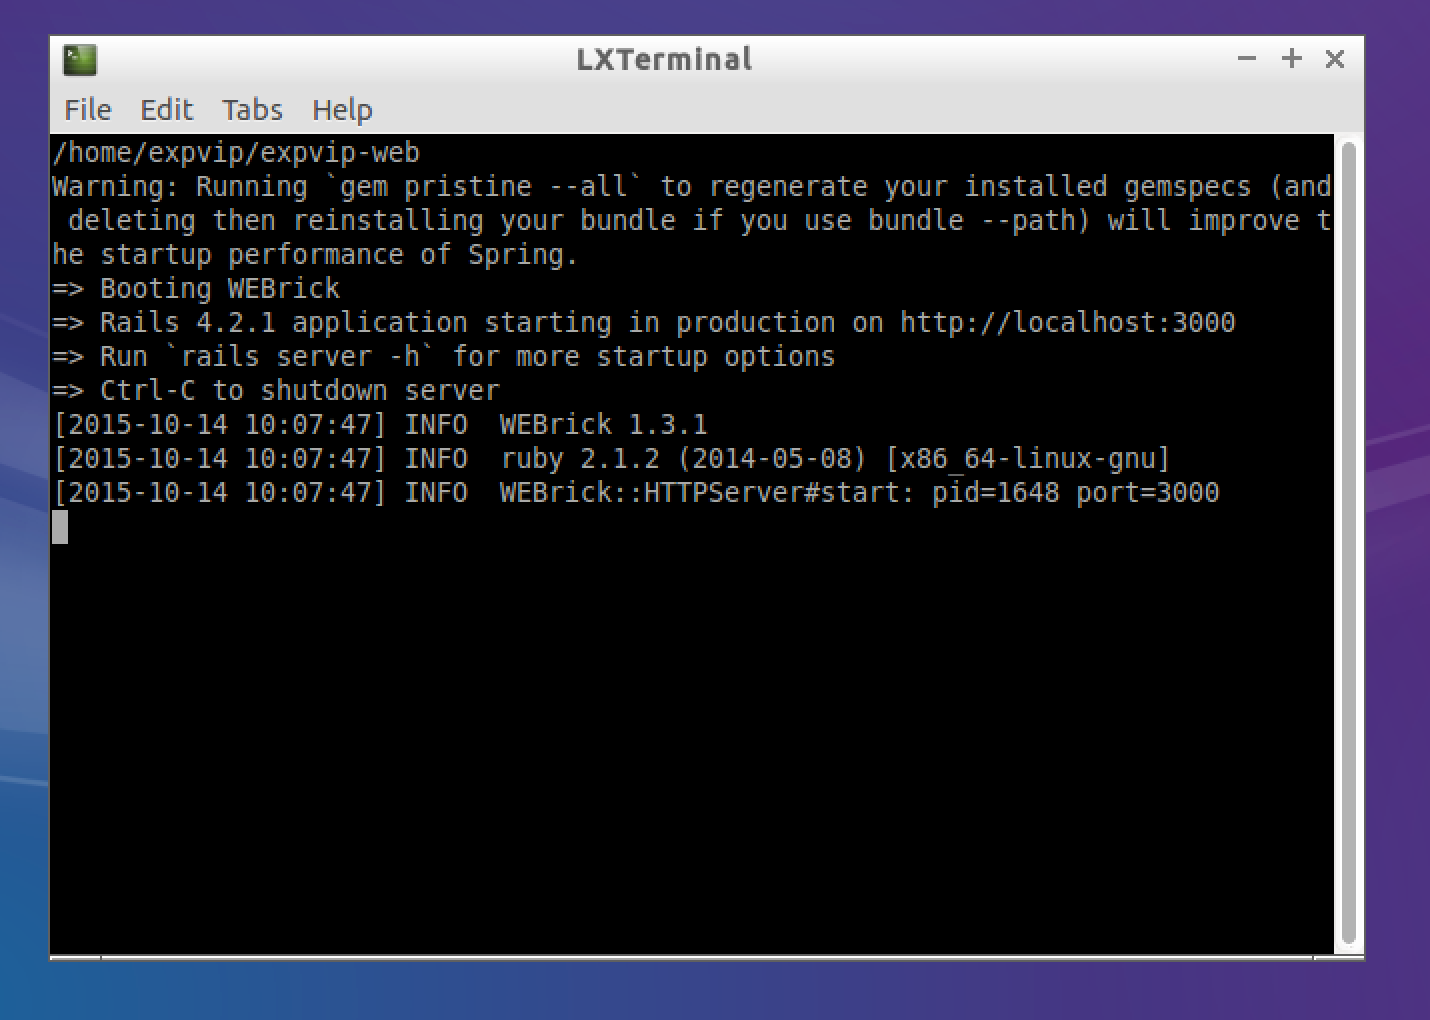
\includegraphics{images/StartupServer03.png}
\item
  Double click in Chromium Web Browser.
  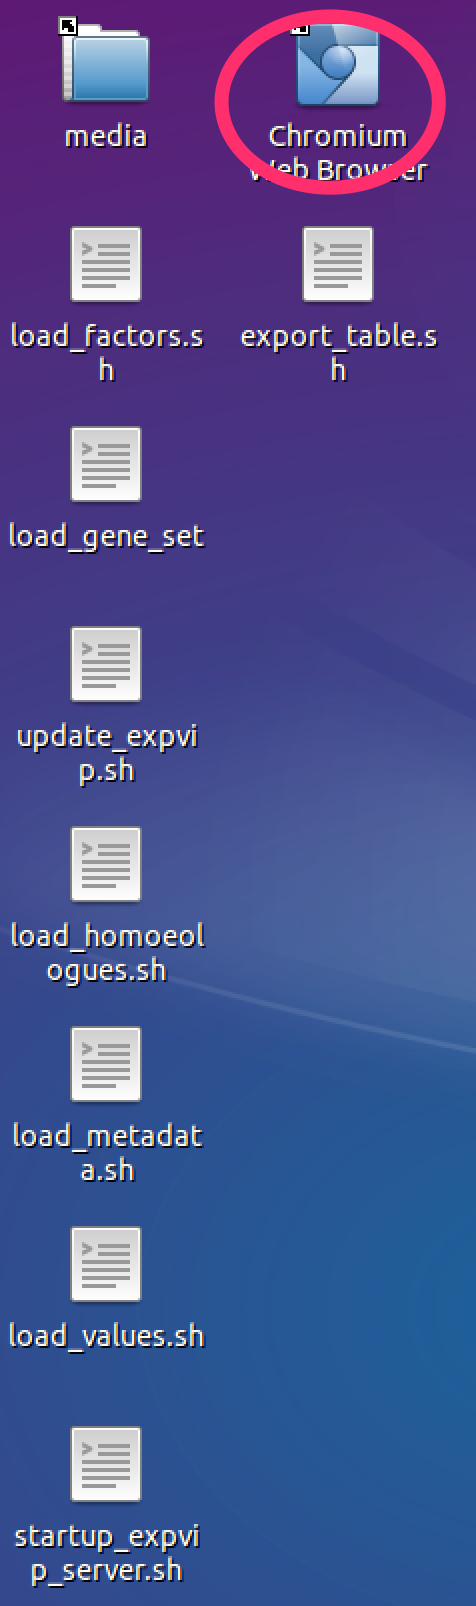
\includegraphics{images/StartupServer04.png}
\item
  Your local instance of expVIP is running!
  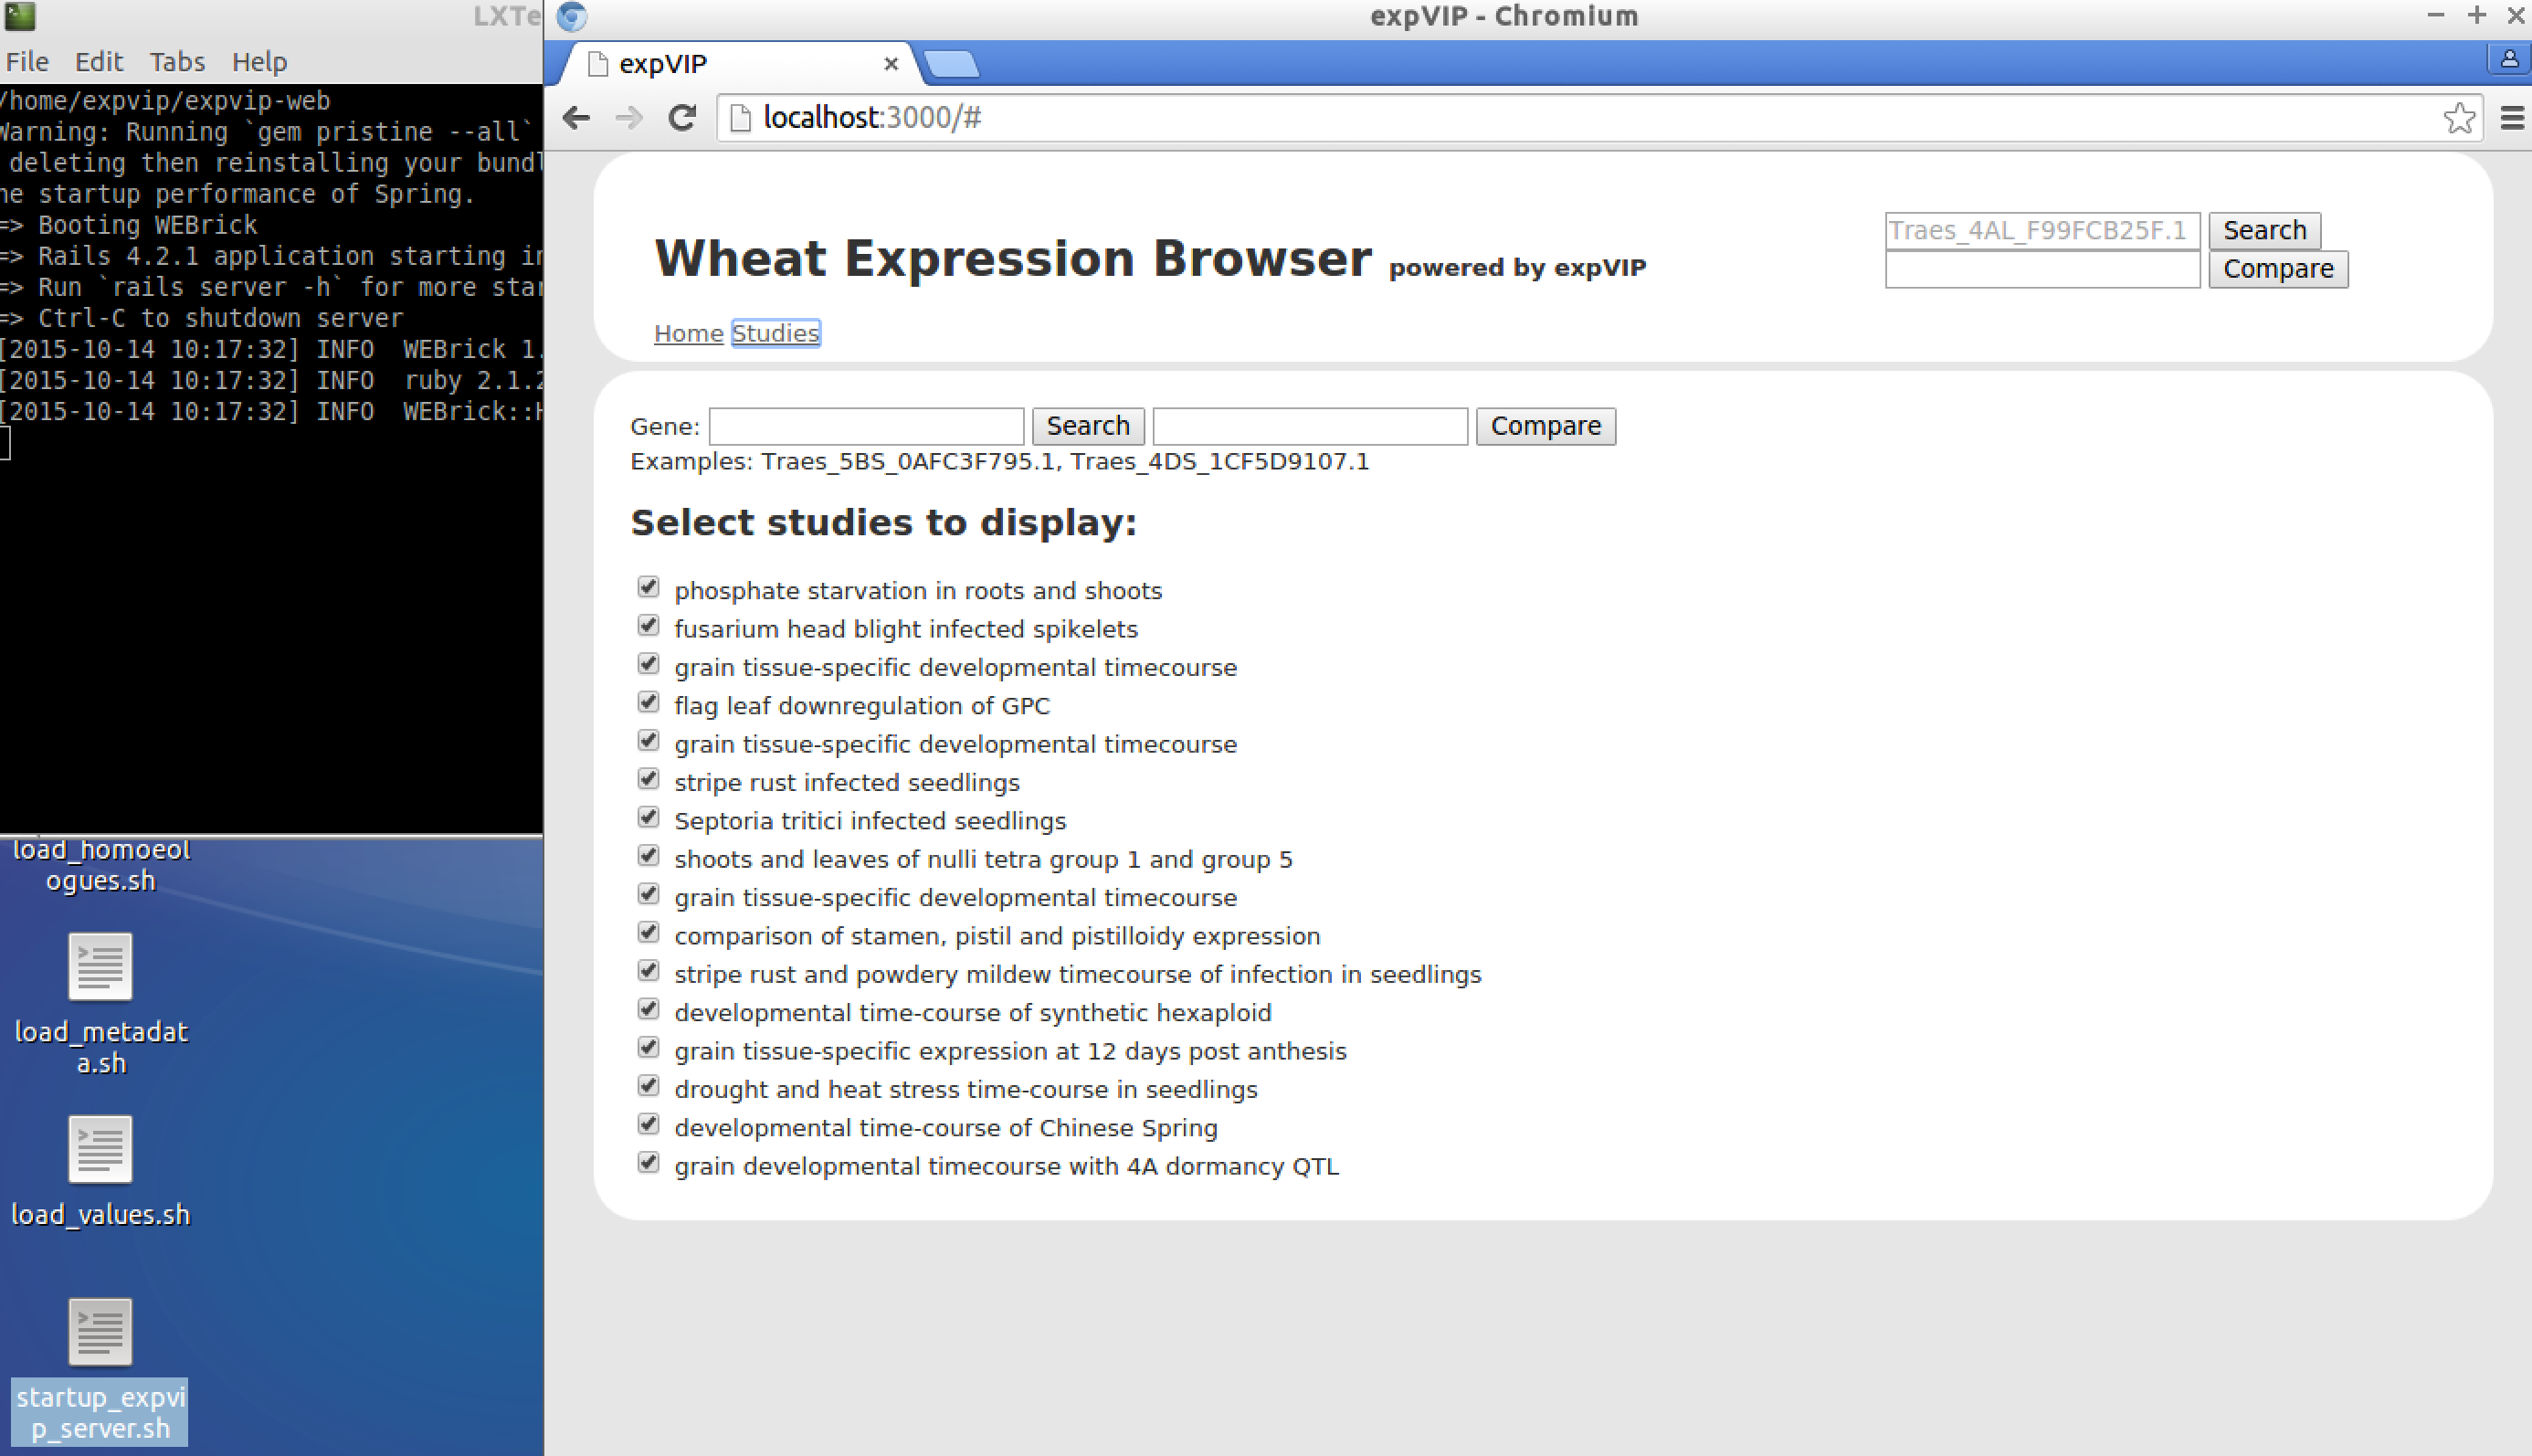
\includegraphics{images/StartupServer05.png}
\end{enumerate}
